\subsection{Estimation methods}
% 3 pages
Estimating the extent of tasks is always relevant, as it (obviously) gives an idea of how long each task probably will take to finish. Even though one does not always actively make these estimations on a small project/task, one does always have an idea of how long the individual tasks will take.

The knowledge is essential to plan a project, because the sum of all estimations sheds light on how long time the project probably will take, which in turn enables several different planning methods to be used, each providing an more-or-less optional route through the tasks.

The use of estimation methods allowed us to be precise and thorough in our estimations. Based on the knowledge acquired from the application of the methods, we could make more precise plans to help us overcome the derailed project.

In the following we will present the methods we have used to estimate our tasks for the project, and describe our thoughts on how we experienced the use of these.

\subsubsection{Planning Poker}
Multiple estimation methods exists, but for this part of the project, we have chosen to use Planning Poker, also know as SCRUM Poker, to estimate the remaining tasks.

In Planning Poker, an identical deck of estimation cards is given to each `player'. Each card represents lengths in some selected estimation unit, such as man hours or story points. The cards usually follows the fibonacci sequence (0, 1, 2, 3, 5, 8, 13, ...) since tasks becomes increasingly harder to estimate accurately as they grow in size.
To `play', two or more players are needed in addition to a moderator. The role of the moderator is to keep the game productive and focused, while the role of the players is to estimate tasks.
For each task, a game of Planning Poker is played, each consisting of up to multiple rounds. A game is played as explained below \cite[p. ?]{?}:
\begin{enumerate}
	\item The moderator starts each game by providing a short overview of the task. The players are able to ask questions and discuss to clarify assumptions and risks. During discussions, no player should express how long the task will take, or how `easy' the task is, as it will influence the estimates of other player subconsciously.
	\item Next each player selects the card from their deck which matches their estimate best, and when all players are ready, all selected cards are revealed at the same time.
	\item If the same estimation is not given by the players, the players with the highest and lowest estimates both justifies their estimate, after which the discussion continues.
	\item Repeat from step two until consensus is reached.
\end{enumerate}

Planning Poker is considered a good practice when using SCRUM \cite[p. ?]{?}. It is also a part of the WBS/PBS paradigm (in SCRUM it is the backlog). [ TODO: Give a brief explaination of WBS/PBS ]

Planning Poker seemed like a good choice since we all have worked with SCRUM before, but not used Planning Poker. Now was a great opportunity to practice it.

The fact that the players do not influence each other when estimating, while the game still facilitates shorts discussion, gives Planning Poker an advantage over traditional, discussion-only estimation \cite[p. ?]{?}. 
The fact that the `game' facilitates discussions is the reason for why we chose Planning Poker over the Delphi estimation method, which does not.

The discussion might not always be an advantage, though. It can easily become very time consuming. We chose a non-voting, but overruling, moderator to address this potential problem, and we believe it worked great proving an advantage multiple times.

\begin{figure}[H]
%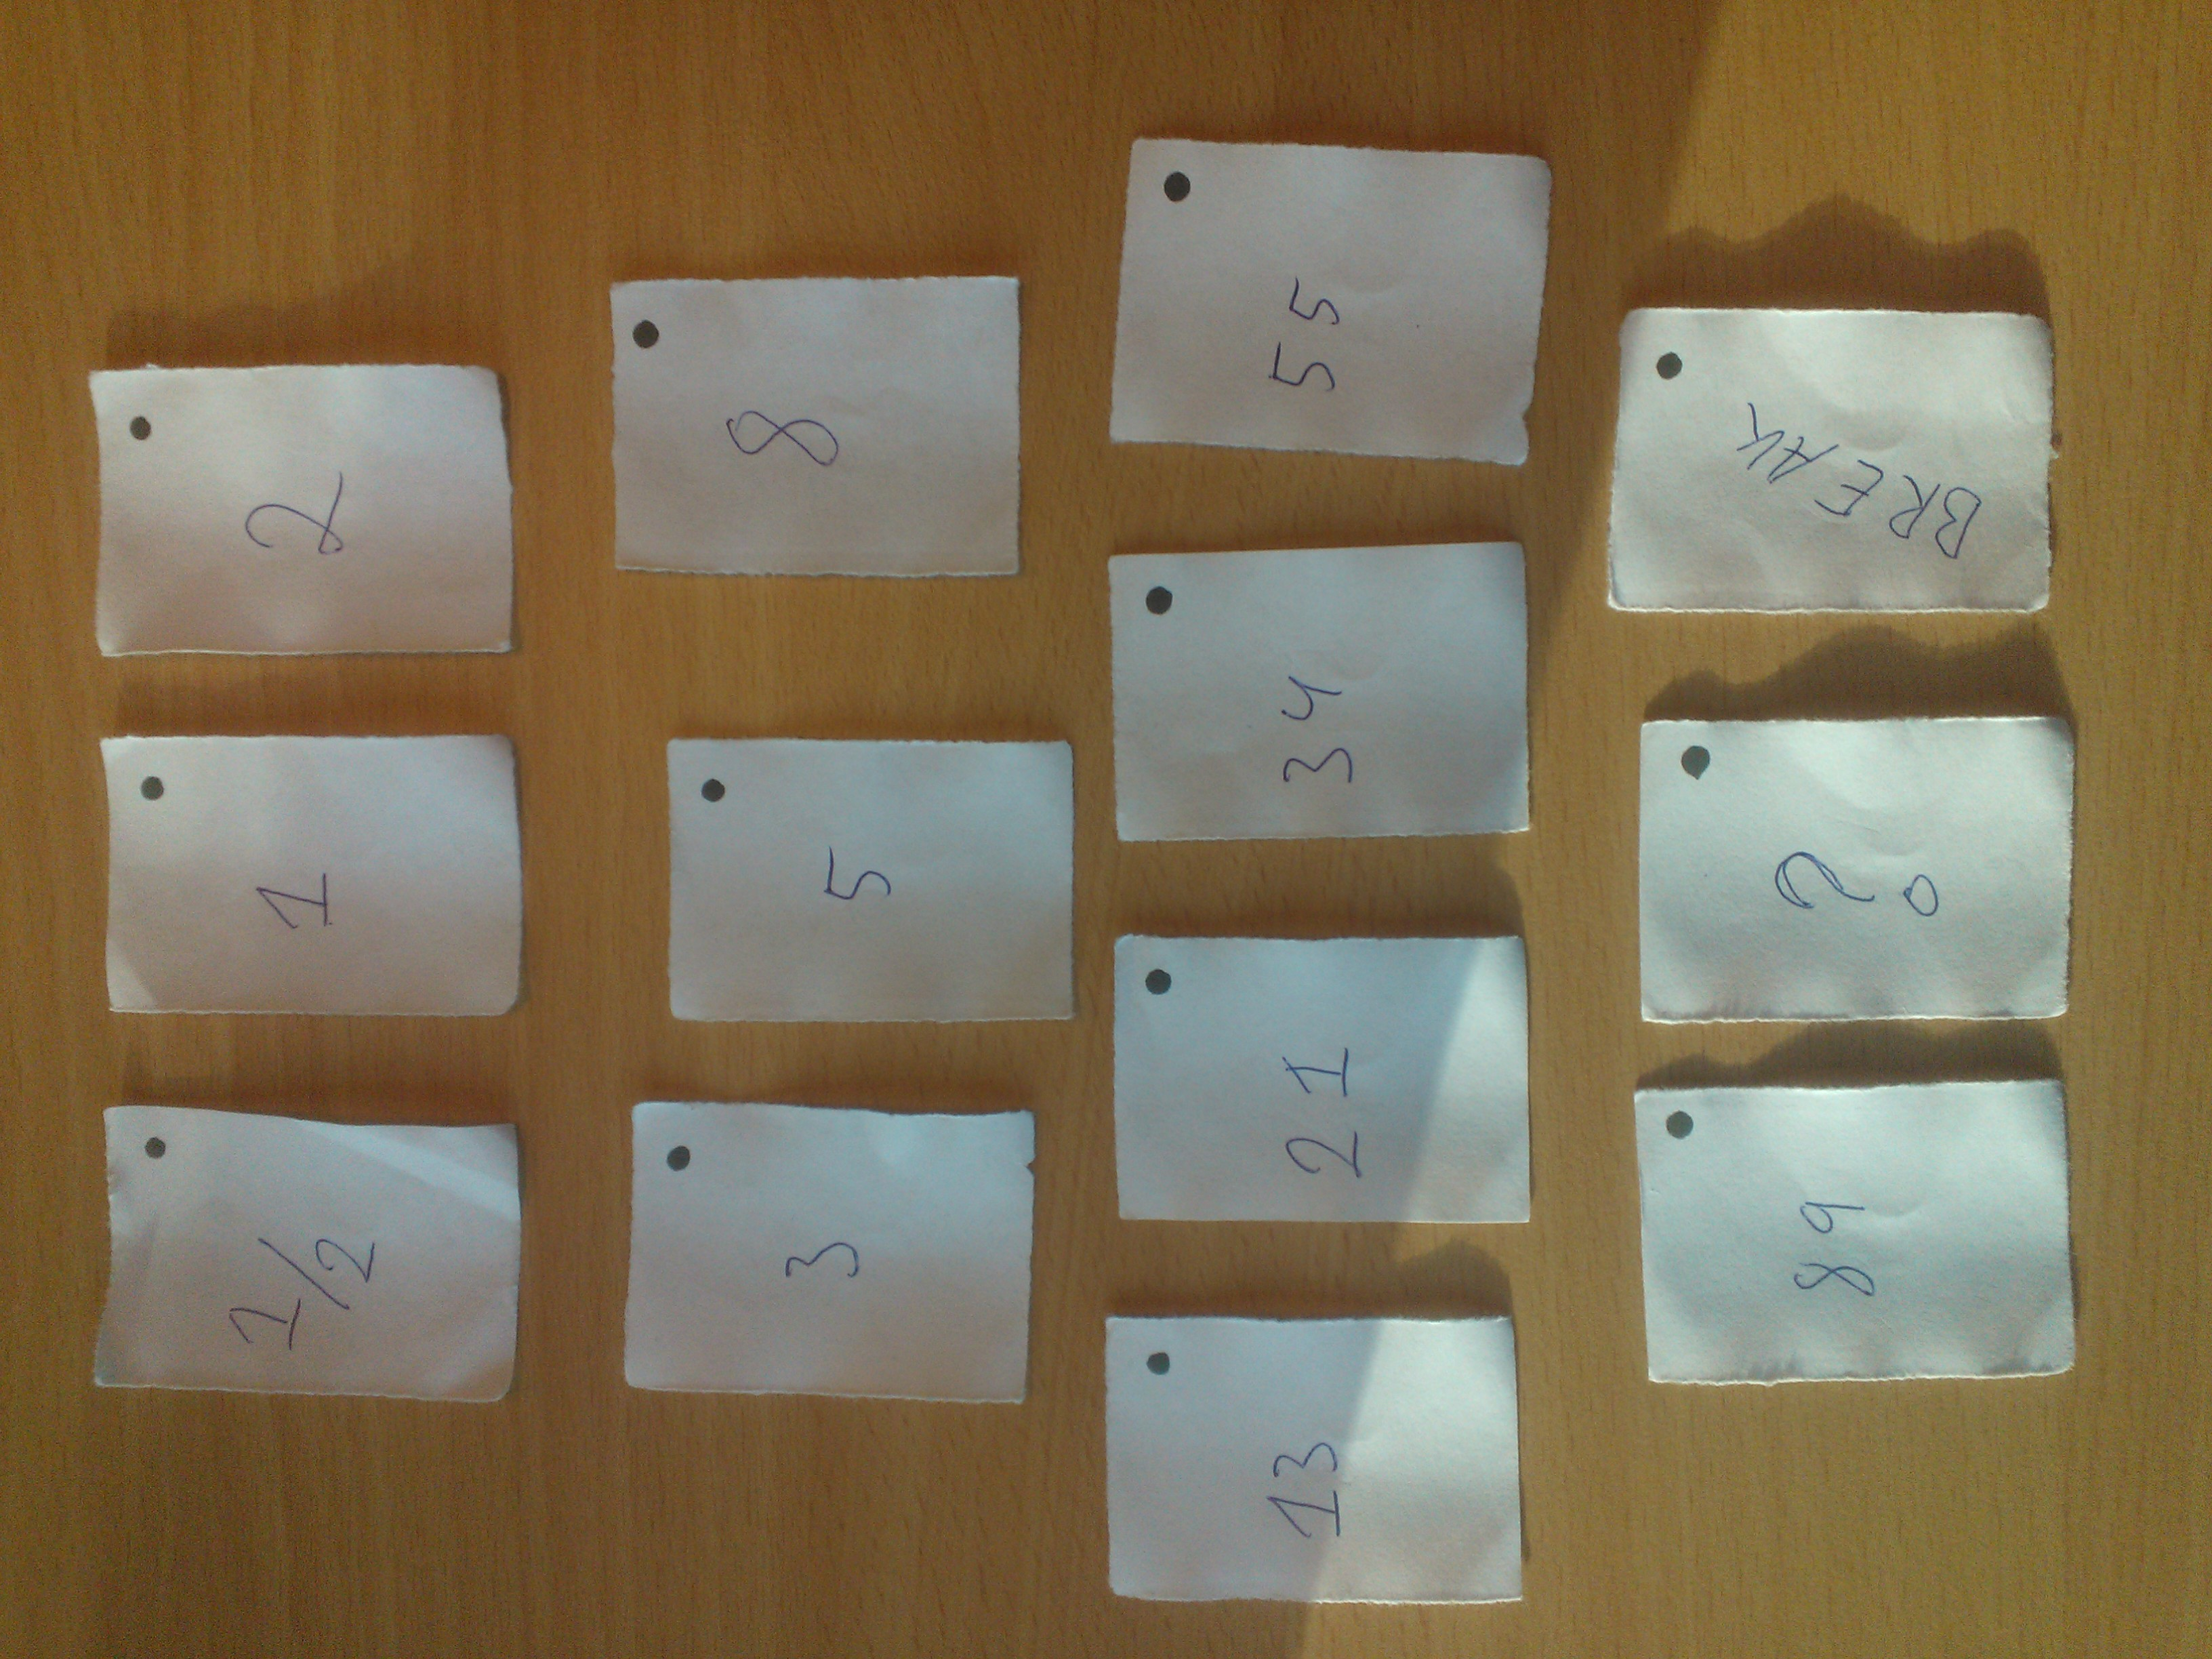
\includegraphics[width=\textwidth,natwidth=2157,natheight=1336]{illustrations/scrumPokerCards.jpg}
  \caption{Scrum poker cards}
  \label{scrumPokerCards}
\end{figure}

For our games we made playing cards with the numbers 1/2, 1, 2, 3, 5, 8, 13, 21, 34, 55, 89, `?' and `break'. The numbers represented man hours and the question-mark represented that the `player' was unable to give a good estimate, while the "break" card represented that the player needed a short break from the game.

We found that using Planning Poker had several advantages over to what we previously had done. Beside the work-related advantages we also found it way more motivating than other methods, and all members of the group was included in the process. Yet, the high numbers (55 and 89) was never used, as well as the `break' card. The `?' was only rarely used, and at last not considered a valid card by the team, due to the fact that when playing the card the player did not participate in the discussion. Also it introduced the risk of only one person having a real estimation vote for the task.

\subsubsection{CoCoMo estimation}
CoCoMo is an algorithmic software cost estimation method. With basic CoCoMo one can calculate time estimations depending on the size of the team and the experience of the team, combined with estimated Kilo Lines Of Code (KLOC) and factoring the programming language. It can also be used in other ways. Estimating the other variables, the remaining variable can be calculated, for example cost of project or team size required. One can add many more factors to the CoCoMo calculation: Complexity, reliability, hardware constraints and more.

We have chosen not to use the CoCoMo estimation. We do not have enough known variables to compute an estimate that is more accurate than user Planning Poker. Planning Poker also force us to discuss each backlog item, as we disagree upon the estimation. The time spend discussing, pulls the team together on the same page. 

\subsubsection{PERT estimation}
A last estimation method we have thought about is the PERT estimation method. While most other methods only ends up with one estimation for each task, the PERT method uses 3 estimates, and then calculate it into one. The force of the PERT method lies in its 3 estimates:
\begin{enumerate}[label=\Alph{*}\hspace{0.8em}]
	\item The optimistic estimate
	\item The realistic estimate
	\item The pessimistic estimate
\end{enumerate}
Then with the use of a the following formula, the end-estimate is calculated.
\begin{equation}
	\frac{A+4B+C}{6}
\end{equation}

We did not use the method, due to the fact that we had already used the Planning Poker method.\\
Looking back it would definitely have been a possibility to combine the Planning Poker method with the PERT method. Instead of each player only turning one card, they turns 3 cards. A optimistic estimate, a realistic estimate and a pessimistic estimate. So instead of having to agree on one estimate, the `players' would have to agree on all 3 estimates.